\documentclass[11pt]{article}

\usepackage[utf8]{inputenc}
\usepackage[T1]{fontenc}
\usepackage{lmodern}
\usepackage[margin=1in]{geometry}
\usepackage{microtype}
\usepackage{amsmath,amssymb,amsthm,mathtools}
\usepackage{graphicx}
\usepackage{booktabs}
\usepackage{array}
\usepackage{ragged2e}
\usepackage{float}
\usepackage{xcolor}
\usepackage{csquotes}
\usepackage{natbib}
\usepackage[hidelinks]{hyperref}
\usepackage[capitalise,nameinlink]{cleveref}
\hypersetup{
  pdftitle={Operator-Level Boolean Computation with Correspondence Matrices},
  pdfauthor={Brian Theory},
  pdfsubject={Typed Boolean operator alignment, fusion, and logical pairing},
  pdfkeywords={Boolean logic, correspondence matrices, operator fusion, logical matrices, compiler optimization}
}

\graphicspath{{../04_figures/}}
% Operator notation for the new Correspondence Matrices manuscript.
% Requires amsmath for bmatrix in the convenience macros below.

\makeatletter
\newbox\impax@lr
\newbox\impax@ud

% Optional optical adjustments; keep at zero unless a manuscript font requires
% a small correction after rendered inspection.
\newcommand{\impaxHtweak}{0pt}
\newcommand{\impaxVtweak}{0pt}

\newcommand{\impax@draw}[2]{%
  \setbox\impax@lr\hbox{$\m@th#1\Leftrightarrow$}%
  \setbox\impax@ud\hbox{$\m@th#1\Updownarrow$}%
  \hbox{%
    \copy\impax@lr
    \kern-\wd\impax@lr
    \hbox to\wd\impax@lr{\hss
      \kern\impaxHtweak
      \raise\impaxVtweak\box\impax@ud
    \hss}%
  }%
}

\newcommand{\impax}{\mathrel{\mathpalette\impax@draw\relax}}
\makeatother

\providecommand{\otbktwo}[2]{\left|#1\right\rangle\!\left\langle#2\right|}
\providecommand{\inbkthree}[3]{\left\langle#1\middle|[#2]\middle|#3\right\rangle}
\providecommand{\twobytwo}[4]{%
  \begin{bmatrix}#1 & #2 \\ #3 & #4\end{bmatrix}%
}


\newcommand{\Bool}{\mathbb{B}}
\newcommand{\GFtwo}{\operatorname{GF}(2)}
\newcommand{\Formula}{\mathcal{F}}
\newcommand{\XOR}{\mathbin{\Updownarrow}}
\newcommand{\CM}[1]{[#1]}
\newcommand{\stateket}[1]{\left|#1\right\rangle}
\newcommand{\statebra}[1]{\left\langle#1\right|}
\DeclareMathOperator{\vecop}{vec}
\DeclareMathOperator{\rot}{rot}
\newcolumntype{L}[1]{>{\RaggedRight\arraybackslash}p{#1}}

\newtheorem{proposition}{Proposition}
\newtheorem{theorem}{Theorem}
\newtheorem{lemma}{Lemma}

\title{Operator-Level Boolean Computation with Correspondence Matrices}
\author{Brian Theory}
\date{}

\begin{document}
\maketitle

\begin{abstract}
Correspondence matrices (CMs) encode binary logical connectives as
$2\times2$ Boolean operators in a declared operand frame. Their purpose is not
merely to reshape the four values of a truth table. Once the operand encoding
and scalar algebra are fixed, a CM can be evaluated, transformed to account
for operand order and polarity, and fused with other operator matrices before
the operands themselves are evaluated. We define CM evaluation as an
XOR--AND contraction over $\GFtwo$: conjunction replaces arithmetic
multiplication and exclusive-or, written $\XOR$, replaces arithmetic addition.
True-first one-hot bras and kets make this contraction select exactly the
connective value associated with the two operands. We then distinguish
linearity in the operator coefficients from linearity of a Boolean function
in its inputs, derive the row, column, and transpose transformations induced
by signed operand changes, and state the condition under which pointwise
operator fusion is sound. A formula-valued logical matrix (LM) provides a
symbolic lift: positive valuation produces the corresponding numeric CM, and
valuation commutes with Boolean operations and the LM pairing. This separates
LMs from algebraic-normal-form coefficients and from semi-tensor-product
logical structure matrices. Together, these results provide the typed
foundation for a compiler method that normalizes compatible operand frames
and performs verified operator-level fusion. The empirical part of the study
is specified by a protocol that must be frozen before execution; it asks when
this rewrite saves total work after compilation, memory, and interface costs
are included. No performance result is claimed before that campaign is
completed.
\end{abstract}

% Draft status: the formal and expository core is being drafted before the
% frozen empirical campaign. No quantitative performance claim is made here.

\section{Introduction}
\label{sec:introduction}

Boolean computation is usually written as a sequence of operations on truth
values or as a symbolic expression whose internal nodes are logical
connectives. Either view makes the operands prominent and leaves each
connective as a small instruction attached to an expression node. A
correspondence matrix reverses that emphasis. It packages a binary connective
as a $2\times2$ operator whose rows and columns are indexed by the states of
its two operands. Once those axes are declared consistently, the operator can
be evaluated, transformed, and combined as an object in its own right.

This operator interpretation is the essential point of the construction. A
CM contains the same four output bits as a binary truth table, so its
information content is not new. What changes is how those bits participate in
computation. A true-first bra for the left operand, a CM in the middle, and a
true-first ket for the right operand form a Boolean contraction. Because both
states are one-hot, the contraction selects exactly one matrix entry. The
matrix therefore acts as the connective rather than merely displaying it.

The same view becomes useful before evaluation. Transposition exchanges the
operands, row or column permutations absorb input negations, and entrywise
complement negates the output. These transformations can place two operator
occurrences into an identical \emph{operand frame}: the same variables, axis
order, polarity, and truth-state convention. When the frames agree, an outer
Boolean connective can be applied entrywise to the two CMs. The resulting CM
replaces the two subexpressions without changing their value. The compiler
question is therefore not whether a truth table can be reshaped, but whether
operator normalization and fusion can remove repeated work often enough to
repay their preparation and representation costs.

Matrix treatments of logic have a substantial history. Boolean matrix
algebras were developed for computer manipulation of logical functions well
before CMs \citep{edwards1972}. Matrix logic and vector logic treat logical
connectives as operators, including outer-product operator bases and matrices
acting on Kronecker products of truth vectors \citep{stern1988,mizraji1992,
mizraji2008}. Semi-tensor-product work gives numeric logical structure
matrices for Boolean functions and network dynamics
\citep{chengqi2010,zhaogaocheng}, while \citet{chengzhaoxu2011} explicitly
uses Boolean matrix operations with XOR as addition and AND as multiplication.
Accordingly, this paper does not claim that truth tables, Boolean matrix
products, logical matrix operators, or pointwise combination of truth values
are new.

The contribution of this paper is narrower and computationally testable: a
typed pipeline that represents a binary connective as a compact CM, records
its operand frame, aligns signed variable pairs through explicit matrix
transformations, fuses only exact compatible frames, and exposes a fallback
when structural fusion is unavailable. The mathematical identities are
elementary or antecedented; their role is to make the compiler transformation
precise enough to prove and measure. The paper makes the following
contributions.

\begin{enumerate}
  \item It defines CM evaluation as XOR--AND contraction over $\GFtwo$ and gives
  a typed operand-frame calculus for exchange, polarity, and sound
  same-operands fusion.
  \item It specifies and proves distinct pure-structural, hybrid,
  whole-expression retabulation, and ordinary-fallback compiler outcomes.
  \item It defines formula-valued LMs, proves their valuation and
  logical-pairing properties, and separates them from ANF and STP coordinate
  representations.
  \item It specifies a reproducible empirical boundary test that counts
  preparation, compilation, memory, query, and interface costs against direct
  packed, sharing-aware, ROBDD, and AIG comparators.
\end{enumerate}

An earlier public manuscript introduced Correspondence Matrices under the
author's former name \citep{droncheff2018}. The present work is a substantial
revision rather than a republication of that text. It narrows the novelty
claim, makes the scalar algebra and basis order explicit, replaces the earlier
higher-dimensional size formulas with the correct $2^n$ entry count, removes
the proposed equivalence with ordinary modulo, and treats measurement and
superposition only as nonphysical Boolean operations. It also adds the
operand-alignment compiler rule, a versioned correctness argument, and a new
evaluation designed to report positive, neutral, and negative performance
regions.

The remainder first defines CM operators and their evaluation semantics, then
presents operand alignment, fusion, and the compiler. It next compares the
construction with matrix logic, STP, ANF, and small-function synthesis before
developing formula-valued LMs as a secondary symbolic extension. All theory
therefore precedes the experimental method, evidence status, discussion, and
conclusion. Detailed proofs and finite-check scopes appear in the appendix.

\section{Correspondence matrices as Boolean operators}
\label{sec:cm-operators}

\subsection{States, axes, and scalar algebra}

Let $\Bool=\{0,1\}$. We write conjunction as $\wedge$, negation as $\neg$,
and exclusive-or as $\XOR$.\footnote{The paper uses $\XOR$
(\texttt{\textbackslash Updownarrow}) rather than a circled-plus glyph. In
the declared true-first frame, the XOR CM is a $90^\circ$ rotation and the
entrywise complement of the XNOR CM. Rotating the XNOR glyph visually gives
the chosen XOR glyph, and overlaying the two motivates the Impax glyph used
below.} When bits are regarded as elements of $\GFtwo$, multiplication is
conjunction and addition is exclusive-or. Every displayed CM contraction uses
this algebra. It is not an arithmetic matrix product over the integers, reals,
or complex numbers.

For $x\in\Bool$, define the true-first state
\begin{equation}
  \stateket{x}=\begin{bmatrix}x\\ \neg x\end{bmatrix},
  \qquad
  \statebra{x}=\begin{bmatrix}x&\neg x\end{bmatrix}.
  \label{eq:true-first-state}
\end{equation}
The first component represents truth and the second represents falsity. CM
rows are ordered by the left operand $X=1,0$, and columns by the right operand
$Y=1,0$. This declared order is part of the type of the representation; a
software array using another order must be converted explicitly.

For a binary operator $\Theta:\Bool^2\rightarrow\Bool$, define
\begin{equation}
  \CM{\Theta}
  :=
  \begin{bmatrix}
    \Theta_{11} & \Theta_{10}\\
    \Theta_{01} & \Theta_{00}
  \end{bmatrix}
  =
  \begin{bmatrix}
    1\mathbin{\Theta}1 & 1\mathbin{\Theta}0\\
    0\mathbin{\Theta}1 & 0\mathbin{\Theta}0
  \end{bmatrix}.
  \label{eq:cm-definition}
\end{equation}
Thus $\Theta_{xy}:=x\mathbin{\Theta}y$ denotes one matrix entry. The bare
bracketed operator, such as $\CM{\XOR}$, names a particular CM; $\CM{\Theta}$
is the generic form. There is no function subscript on the whole matrix in the
main-text notation because the operator itself already supplies the needed
identity.

\subsection{XOR--AND contraction}

For any $C\in\Bool^{2\times2}$, define
\(\chi_x(r)=1\) when \(r=x\) and \(\chi_x(r)=0\) otherwise. The row and
column state encodings have this same component function. Then
\begin{equation}
  E_C(x,y)
  :=\statebra{x}C\stateket{y}
  :=\mathop{\XOR}_{r,s\in\{1,0\}}
       \chi_x(r)\wedge C_{rs}\wedge\chi_y(s).
  \label{eq:boolean-contraction}
\end{equation}
Equation~\eqref{eq:boolean-contraction} is a Boolean contraction: AND forms
each term and XOR reduces the four terms. The compact bra--operator--ket
notation suppresses those mechanics after they have been declared.

\begin{proposition}[CM selection]
For every binary Boolean operator $\Theta$ and $x,y\in\Bool$,
\begin{equation}
  \statebra{x}\CM{\Theta}\stateket{y}
  =x\mathbin{\Theta}y.
  \label{eq:selection}
\end{equation}
\end{proposition}

\begin{proof}
Each state in \eqref{eq:true-first-state} has exactly one nonzero component.
In the four-term contraction, every term except the one indexed by $(x,y)$
therefore contains a zero factor. The surviving term is
$1\wedge\Theta_{xy}\wedge1=\Theta_{xy}$.
\end{proof}

For XOR, the operator matrix is
\begin{equation}
  \CM{\XOR}=\begin{bmatrix}0&1\\1&0\end{bmatrix}.
\end{equation}
Taking $x=1$ and $y=0$ gives
\begin{equation}
  \statebra{1}\CM{\XOR}\stateket{0}
  =\begin{bmatrix}1&0\end{bmatrix}
   \begin{bmatrix}0&1\\1&0\end{bmatrix}
   \begin{bmatrix}0\\1\end{bmatrix}
  =1,
\end{equation}
where the displayed products and reduction retain the AND/XOR meaning of
\eqref{eq:boolean-contraction}. Figure~\ref{fig:cm-evaluation} presents the
same evaluation visually and introduces the geometric notation used below.

\begin{figure}[t]
  \centering
  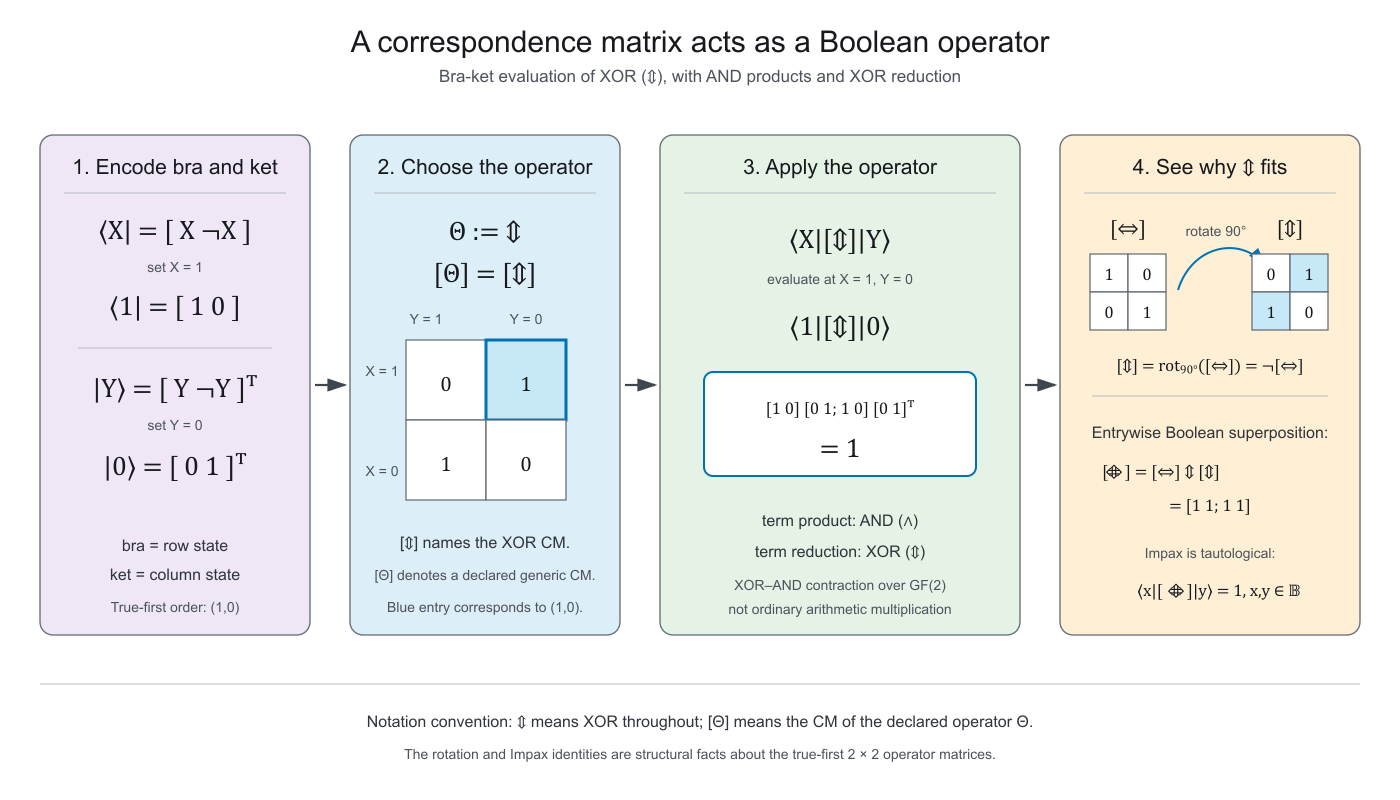
\includegraphics[width=\textwidth]{figure_01_boolean_operator_contraction_preview.png}
  \caption{A binary truth value is encoded as a true-first bra or ket, and
  $\CM{\Theta}$ acts between them through XOR--AND contraction. The XOR CM
  $\CM{\XOR}$ is a $90^\circ$ rotation and entrywise complement of the XNOR
  CM $\CM{\Leftrightarrow}$. Their entrywise Boolean superposition is the
  tautological Impax CM $\CM{\impax}$.}
  \label{fig:cm-evaluation}
\end{figure}

\subsection{Coefficient-space linearity}

The contraction is linear in the four operator coefficients over $\GFtwo$.
For fixed $x$ and $y$ and matrices $A,B\in\Bool^{2\times2}$,
\begin{equation}
  E_{A\XOR B}(x,y)=E_A(x,y)\XOR E_B(x,y),
  \qquad E_0(x,y)=0,
  \label{eq:coefficient-linearity}
\end{equation}
where $A\XOR B$ is entrywise XOR. This statement is deliberately narrow. It
does not say that the Boolean function represented by a CM is linear in $x$
and $y$. Nor does it make the state encoding linear: the map
$x\mapsto[x,\neg x]^\mathsf{T}$ is affine because it sends $0$ to
$[0,1]^\mathsf{T}$ rather than the zero vector. If the contraction is extended
to arbitrary vectors in $\GFtwo^2$, it is separately linear in the bra, the
matrix coefficients, and the ket; that multilinearity remains distinct from
the algebraic degree of the represented Boolean function.

Let $E_{rs}$ contain a one at position $(r,s)$ and zeros elsewhere. The four
matrices $E_{11},E_{10},E_{01},E_{00}$ form the standard basis of
$\GFtwo^{2\times2}$, and
\begin{equation}
  \CM{\Theta}
  =\mathop{\XOR}_{r,s\in\{1,0\}}\Theta_{rs}E_{rs}.
  \label{eq:operator-basis}
\end{equation}
Equation~\eqref{eq:selection} extracts the corresponding coefficient. This is
a minterm-indicator or operator-basis expansion, not the algebraic normal form
of $\Theta$ in uncomplemented variables.

\subsection{XNOR, XOR, and Impax}

The true-first XNOR and XOR matrices are
\begin{equation}
  \CM{\Leftrightarrow}=\begin{bmatrix}1&0\\0&1\end{bmatrix},
  \qquad
  \CM{\XOR}=\begin{bmatrix}0&1\\1&0\end{bmatrix}.
\end{equation}
Consequently,
define the clockwise rotation of a displayed $2\times2$ array by
\[
  \rot_{90^\circ}\!\begin{bmatrix}a&b\\c&d\end{bmatrix}
  :=\begin{bmatrix}c&a\\d&b\end{bmatrix}.
\]
For this particular pair of operators,
\begin{equation}
  \CM{\XOR}
  =\rot_{90^\circ}\!\left(\CM{\Leftrightarrow}\right)
  =\neg\CM{\Leftrightarrow}.
  \label{eq:xor-xnor-rotation}
\end{equation}
The Impax operator is the tautological operator represented by the centered
overlay glyph $\impax$. Entrywise Boolean XOR gives
\begin{equation}
  \CM{\impax}
  =\CM{\Leftrightarrow}\XOR\CM{\XOR}
  =\begin{bmatrix}1&1\\1&1\end{bmatrix},
  \qquad
  \statebra{x}\CM{\impax}\stateket{y}=1
  \quad(x,y\in\Bool).
  \label{eq:impax}
\end{equation}
Here \emph{superposition} refers only to the entrywise Boolean operation in
\eqref{eq:impax}; it does not denote a quantum state.

\section{Operand transformations and aligned fusion}
\label{sec:alignment-fusion}

A CM occurrence is typed by an operand frame: its row variable, column
variable, input polarities, and truth-state order. Let
$P=\begin{bmatrix}0&1\\1&0\end{bmatrix}$. With the true-first axes of
\eqref{eq:cm-definition}, define $\Theta^\tau(x,y):=\Theta(y,x)$. Operand
exchange, input negation, and output negation then act as
\begin{align}
  \CM{\Theta^\tau} &= \CM{\Theta}^{\mathsf T}, &
  \CM{\Theta(\neg X,Y)} &= P\CM{\Theta},\\
  \CM{\Theta(X,\neg Y)} &= \CM{\Theta}P, &
  \CM{\neg\Theta} &= \mathbf{1}\XOR\CM{\Theta}.
  \label{eq:frame-transformations}
\end{align}
The matrix products involving $P$ are XOR--AND products; here they simply
permute rows or columns. They are not a general NPN canonicalizer. Their role
is to rewrite an admitted signed pair into one explicitly declared operand
frame.

For a binary outer operator $\Phi$, define entrywise fusion by
\begin{equation}
  (\CM{\Theta_1}\mathbin{\Phi}\CM{\Theta_2})_{rs}
  :=(\Theta_1)_{rs}\mathbin{\Phi}(\Theta_2)_{rs}.
\end{equation}
If both matrices act on the same ordered operands in the same frame, then
\begin{equation}
  (x\mathbin{\Theta_1}y)\mathbin{\Phi}(x\mathbin{\Theta_2}y)
  =\statebra{x}
     (\CM{\Theta_1}\mathbin{\Phi}\CM{\Theta_2})
     \stateket{y},
  \qquad x,y\in\Bool.
  \label{eq:same-operands-fusion}
\end{equation}
Both sides select position $(x,y)$, so the identity holds for every binary
$\Phi$ without requiring $\Phi$ to distribute over XOR. Pointwise truth-table
combination is established prior art; the compiler-specific claim is the
typed admission rule that first proves frame agreement and otherwise refuses
this fusion.

\begin{figure}[t]
  \centering
  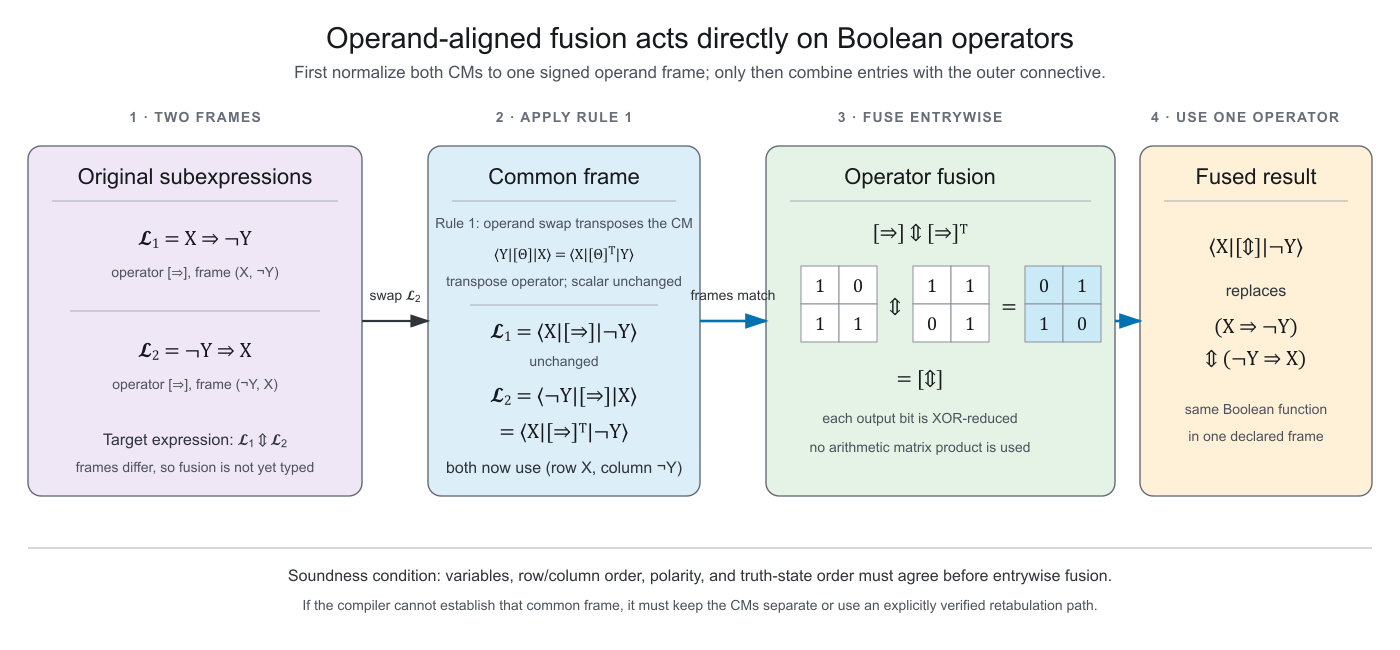
\includegraphics[width=\textwidth]{figure_03_operand_alignment_and_fusion_preview.png}
  \caption{Two operator occurrences are first rewritten into one declared
  operand frame and are then fused entrywise. The transformed bra--operator--ket
  expression records the operand exchange explicitly; fusion is not applied
  while the frames differ.}
  \label{fig:alignment-fusion}
\end{figure}

\subsection{Compiler rule and soundness boundary}

Fix distinct declared variables $R$ and $C$ in disjoint row and column layout
sets, and let $\Gamma=(R,C,F)$ include a fixed-assignment map $F$ that binds
neither $R$ nor $C$ on a returned pair path. Expressions use the grammar
$e::=Z\mid\neg e\mid e\mathbin{\Phi}e$, where $Z$ is a variable and $\Phi$ is
one of the five supported binary connectives. A typed result has judgment
\begin{equation}
  \Gamma\vdash e\Downarrow^{p}\operatorname{Pair}(R,C,t),
  \qquad p\in\{\mathsf{S},\mathsf{R},\mathsf{H}\},
  \label{eq:pair-judgment}
\end{equation}
where $\mathsf{S}$ means purely structural, $\mathsf{R}$ means that the whole
returned subtree was retabulated, and $\mathsf{H}$ means that structural steps
consume at least one retabulated descendant. Every returned token must satisfy
\begin{equation}
  E_t(r,c)=e[r/R,c/C]
  \qquad\text{for all }r,c\in\Bool,
  \label{eq:pair-invariant}
\end{equation}
after applying $F$.

The inference rules are intentionally small. A supported connective over two
signed literals in the declared row/column sets yields provenance
$\mathsf{S}$ after the required transpose and polarity permutations. Negation
complements a child token. Two children may fuse only when their $(R,C)$
metadata agree. In symbols,
\begin{equation}
 \frac{\Gamma\vdash a\Downarrow^p\operatorname{Pair}(R,C,t_a)}
      {\Gamma\vdash\neg a\Downarrow^{\nu(p)}
       \operatorname{Pair}(R,C,\neg t_a)}
 \qquad
 \frac{\Gamma\vdash a\Downarrow^p\operatorname{Pair}(R,C,t_a)\quad
       \Gamma\vdash b\Downarrow^q\operatorname{Pair}(R,C,t_b)}
      {\Gamma\vdash a\mathbin{\Phi}b\Downarrow^{p\sqcup q}
       \operatorname{Pair}(R,C,t_a\mathbin{\Phi}t_b)}.
 \label{eq:pair-rules}
\end{equation}
Here token negation and $\Phi$ are entrywise, $\nu(\mathsf S)=\mathsf S$ and
$\nu(\mathsf R)=\nu(\mathsf H)=\mathsf H$, while
$\mathsf S\sqcup\mathsf S=\mathsf S$ and every other fusion provenance is
$\mathsf H$. If structural construction stops and the live support is exactly
$\{R,C\}$, the optional local rule evaluates all four assignments and returns
provenance $\mathsf R$. The \texttt{pure\_structural} strategy disables that
rule; \texttt{hybrid} enables it; and \texttt{retabulate} bypasses the rules
and retabulates the whole root. Failure to derive a pair selects ordinary IR.

Repeated-variable expressions such as $X\mathbin{\Theta}X$, overlapping
row/column layouts, compound operands treated as opaque, and different
variable pairs remain outside the pure structural rule.

\begin{theorem}[Structural alignment-and-fusion soundness]
If $\Gamma\vdash e\Downarrow^{\mathsf S}\operatorname{Pair}(R,C,t)$, then
\eqref{eq:pair-invariant} holds and no four-assignment retabulation was used.
\end{theorem}

\begin{proof}
Use structural induction over an admitted construction. A signed primitive is
correct by \eqref{eq:frame-transformations}; complementing a correct child
represents negation; and fusing correct children with identical metadata is
sound by \eqref{eq:same-operands-fusion}.
\end{proof}

\begin{lemma}[Exact pair retabulation]
If the live support after fixed substitution is exactly one distinct row
variable $R$ and one distinct column variable $C$, evaluating $e$ at the four
assignments $(1,1),(1,0),(0,1),(0,0)$ produces the unique token satisfying
\eqref{eq:pair-invariant}.
\end{lemma}

\begin{theorem}[Soundness of the admitted pair compiler]
For every derivable provenance $p\in\{\mathsf S,\mathsf R,\mathsf H\}$, a
returned $\operatorname{Pair}(R,C,t)$ satisfies
\eqref{eq:pair-invariant}. Thus pure structural, whole-root retabulation, and
hybrid structural--retabulation results are all sound but remain separately
reported. If no pair judgment is derivable, the ordinary CM IR evaluates the
unchanged expression.
\end{theorem}

\newcommand{\relatedworksection}{%
\section{Related work and representation boundaries}
\label{sec:representation-map}

Several representations considered in this paper carry the same four truth
values, but they are not the same mathematical object. The distinction matters
both for novelty and for correct use of the operations.

The numeric CM $\CM{\Theta}$ is a $2\times2$ Boolean operator in a declared
row/column frame. Its vectorization
\begin{equation}
  \vecop(\CM{\Theta})
  =(\Theta_{11},\Theta_{10},\Theta_{01},\Theta_{00})
  \label{eq:truth-vector}
\end{equation}
is the ordered truth vector, carrying the same four bits in a one-dimensional
layout. To make the STP comparison reproducible, adopt the common delta
encoding $1\mapsto\delta_2^1=[1,0]^\mathsf{T}$ and
$0\mapsto\delta_2^2=[0,1]^\mathsf{T}$, with Kronecker columns ordered
$(11,10,01,00)$. If $t=\vecop(\CM{\Theta})\in\Bool^{1\times4}$ is regarded as
a row vector, the corresponding binary-output structure matrix is then
\begin{equation}
  M_\Theta=
  \begin{bmatrix}
    t\\ \neg t
  \end{bmatrix}.
  \label{eq:stp-conversion}
\end{equation}
where $\neg t$ is the entrywise Boolean complement of $t$.
Other source conventions require an explicit row or column permutation
\citep{chengqi2010,zhaogaocheng}. The $2\times4$ STP matrix is an external
representation, not a component of a CM.

ANF coefficients are farther removed. For two variables, an algebraic normal
form has the shape
\begin{equation}
  X\mathbin{\Theta}Y
  =a_{\varnothing}\XOR(a_X\wedge X)
   \XOR(a_Y\wedge Y)\XOR(a_{XY}\wedge X\wedge Y).
  \label{eq:anf}
\end{equation}
In the paper's true-first storage order, the Boolean M\"obius conversion is
unambiguous when written componentwise:
\begin{align}
  a_{\varnothing}&=\Theta_{00}, &
  a_X&=\Theta_{00}\XOR\Theta_{10},\\
  a_Y&=\Theta_{00}\XOR\Theta_{01}, &
  a_{XY}&=\Theta_{00}\XOR\Theta_{10}\XOR\Theta_{01}\XOR\Theta_{11}.
  \label{eq:anf-conversion}
\end{align}
Thus $a_\Theta=(a_{\varnothing},a_X,a_Y,a_{XY})$ is a polynomial coordinate
representation, not the entries of the formula-valued LM introduced in
\cref{sec:logical-matrices}. The relevant STP treatment uses Kronecker
products of vectors $[1,x_i]^\mathsf{T}$ to enumerate the square-free monomial
basis and gives a conversion from truth values to those coefficients
\citep{zhaogaocheng}; it does not identify the coefficients with a CM or LM.

Figure~\ref{fig:representation-map} summarizes only the numeric conversion
side of these relationships. Its arrows are declared maps, not claims that the
objects have the same mathematical type. The separate symbolic LM-to-CM map is
shown later in Figure~\ref{fig:lm-valuation}, after the LM is defined.

\begin{figure}[t]
  \centering
  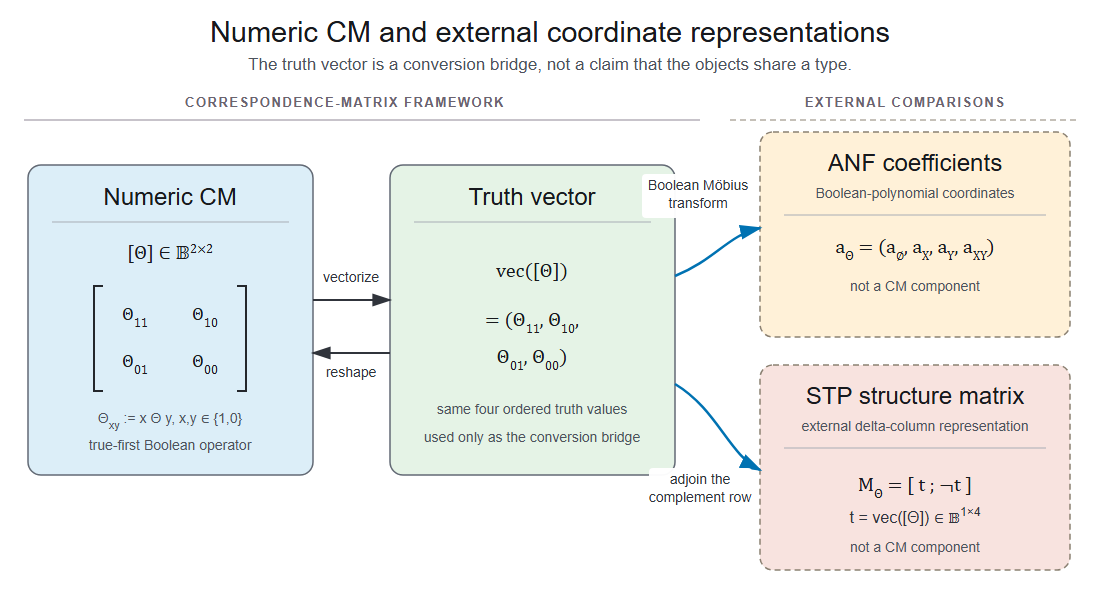
\includegraphics[width=\textwidth]{figure_02_numeric_representation_map_preview.png}
  \caption{Numeric representation boundaries. Vectorization exposes the
  ordered truth values used to compare a CM with ANF coordinates and an STP
  logical structure matrix. ANF and STP are external representations rather
  than CM components. The symbolic LM path is shown separately in
  Figure~\ref{fig:lm-valuation}.}
  \label{fig:representation-map}
\end{figure}

This map also separates three senses of linearity. CM evaluation is linear in
the operator coefficients over $\GFtwo$ for fixed operands
\eqref{eq:coefficient-linearity}. ANF calls a Boolean function linear or
affine when terms of degree greater than one are absent. Matrix and STP
formalisms may additionally be linear in their chosen vector space. None of
these statements implies the others without an explicit conversion and its
domain.

\subsection{Closest operational antecedents}

Small truth functions are routinely stored and manipulated as packed bit
strings in logic synthesis. In the ABC AIG rewriter, for example, four-input
cut functions are stored as 16-bit truth tables, classified up to input
negation, input permutation, and output negation (NPN), and matched to
precomputed replacement DAGs \citep{mishchenko2006}. Modern NPN work likewise
defines equivalence by exactly those transformations and uses canonical or
semicanonical representatives in synthesis and technology mapping
\citep{zhou2019}. These precedents mean that CM transposition, row/column
permutation, complementation, and packed four-bit storage are not individually
new operations.

Logic-synthesis practice also supplies the strongest comparison for the
compiler claim. AIG rewriting preserves and exploits DAG sharing rather than
only the final truth function \citep{mishchenko2006}; broader synthesis flows
move among truth tables, graph networks, and exact or heuristic optimization
according to support size and task \citep{testa2019}. Bit-parallel simulation
packs many assignments into machine words and evaluates a network over those
patterns at once \citep{lee2022}. The present compiler therefore does not
claim a new NPN classifier, LUT mapper, AIG rewriter, or bit-parallel evaluator.
Its candidate contribution is narrower: an explicitly typed two-operand frame
used as an admission certificate for local operator fusion, with a measured
fallback boundary.

\begin{table}[H]
  \centering
  \scriptsize
  \setlength{\tabcolsep}{3pt}
  \begin{tabular}{@{}L{0.14\linewidth}L{0.18\linewidth}L{0.20\linewidth}L{0.20\linewidth}L{0.20\linewidth}@{}}
    \toprule
    Family & Operator/data shape & Scalar algebra & Transform or composition role & Relation to this work \\
    \midrule
    Stern/Mizraji matrix logic & Truth vectors, tensor inputs, matrix gates & Primarily ordinary real/vector algebra & Logical operators and operator bases & Establishes the operator viewpoint and outer-product antecedents \\
    Cheng/Zhao STP and Boolean matrices & $2\times2^n$ structure matrices and Boolean matrices & STP plus explicit XOR--AND Boolean products & Swap/negation matrices and pointwise truth-function combination & Direct overlap with Boolean matrix algebra and fusion identities \\
    ANF & Square-free monomial coefficient vector & $\GFtwo$ polynomial algebra & M\"obius coordinate conversion & Different map and type from a formula-valued LM \\
    NPN/LUT/AIG synthesis & Packed truth tables and shared Boolean DAGs & Bit operations and graph rewrites & Input/output phase, permutation, cut matching, and shared replacement & Closest operational prior art; mandatory baseline family \\
    CM pair compiler & Four-bit token plus declared row/column frame & XOR--AND contraction and entrywise outer connective & Typed signed-frame alignment followed by admitted local fusion & Candidate contribution is the typed integration and measured boundary \\
    \bottomrule
  \end{tabular}
  \caption{Claim boundary against the closest representation and compiler
  families. No row alone establishes novelty; the empirical question concerns
  the integrated typed CM compiler path.}
  \label{tab:related-work-boundary}
\end{table}

}

\newcommand{\logicalmatrixsection}{%
\section{Formula-valued logical matrices}
\label{sec:logical-matrices}

\subsection{Symbolic lift and positive valuation}

Let $\Formula$ be the Boolean algebra of formulas modulo logical equivalence.
Define the polarity orbit
\begin{equation}
  X_1=X,\quad X_2=\neg X,
  \qquad
  Y_1=Y,\quad Y_2=\neg Y.
  \label{eq:polarity-orbit}
\end{equation}
Let $b_1=1$ and $b_2=0$, and reserve $\Theta_{xy}$ for truth assignments
$x,y\in\Bool$. Define the position-indexed LM coefficients by
\begin{equation}
  c_{ij}:=\Theta_{b_i b_j},
  \qquad i,j\in\{1,2\}.
  \label{eq:lm-index-map}
\end{equation}
Thus $(c_{11},c_{12},c_{21},c_{22})$ denotes the same four values as
$(\Theta_{11},\Theta_{10},\Theta_{01},\Theta_{00})$ without overloading one
subscript system. For Boolean coefficients $c_{ij}$, define the formula-valued logical
matrix by the XOR sum of its four polarity outer products:
\begin{equation}
  [\mathcal{M}_{X\Theta Y}]
  :=\mathop{\XOR}_{i,j\in\{1,2\}}
      c_{ij}\,\otbktwo{X_i}{Y_j}.
  \label{eq:lm-outer-product}
\end{equation}
Here $\otbktwo{X_i}{Y_j}$ is the formula-valued outer product
\begin{equation}
  \otbktwo{X_i}{Y_j}
  =\begin{bmatrix}
    X_i\wedge Y_j & X_i\wedge\neg Y_j\\
    \neg X_i\wedge Y_j & \neg X_i\wedge\neg Y_j
  \end{bmatrix}.
  \label{eq:lm-outer-product-expanded}
\end{equation}
Multiplication by $c_{ij}$ means entrywise conjunction. Expanding the XOR sum
gives
\begin{equation}
  [\mathcal{M}_{X\Theta Y}]
  =
  \begin{bmatrix}
    \mathop{\XOR}_{i,j}X_i\wedge c_{ij}\wedge Y_j &
    \mathop{\XOR}_{i,j}X_i\wedge c_{ij}\wedge\neg Y_j\\
    \mathop{\XOR}_{i,j}\neg X_i\wedge c_{ij}\wedge Y_j &
    \mathop{\XOR}_{i,j}\neg X_i\wedge c_{ij}\wedge\neg Y_j
  \end{bmatrix}
  =
  \begin{bmatrix}
    X\mathbin{\Theta}Y & X\mathbin{\Theta}\neg Y\\
    \neg X\mathbin{\Theta}Y & \neg X\mathbin{\Theta}\neg Y
  \end{bmatrix}.
  \label{eq:lm-matrix}
\end{equation}
Thus every cell in \eqref{eq:lm-matrix} is itself a complete XOR-reduced
formula; the four displayed cells are not four separate terms of one formula.
The entries lie in $\Formula$, not
in a numeric vector space. We use \emph{formula-valued LM} to distinguish this
object from the numeric ``logical matrix'' and logical structure matrix of the
STP literature.

A valuation $v:\Formula\rightarrow\Bool$ acts entrywise and preserves
$\neg$, $\wedge$, and $\XOR$. Let $v_T$ be the positive valuation with
$v_T(X)=v_T(Y)=1$. Then
\begin{equation}
  v_T\!\left([\mathcal{M}_{X\Theta Y}]\right)=\CM{\Theta}.
  \label{eq:positive-valuation}
\end{equation}
Under a general valuation $v(X)=x$ and $v(Y)=y$, the result is the same CM with
the row and column permutations determined by $x$ and $y$. If
$P=\begin{bmatrix}0&1\\1&0\end{bmatrix}$, then
\begin{equation}
  v\!\left([\mathcal{M}_{X\Theta Y}]\right)
  =P^{1-x}\CM{\Theta}P^{1-y}.
  \label{eq:general-valuation}
\end{equation}
The LM is therefore a symbolic polarity-orbit matrix whose valuations produce
numeric CMs in declared operand frames. It is not an ANF coefficient vector:
positive valuation, rather than a M\"obius transform, is the map from this LM
to $\CM{\Theta}$.

The present compiler does not manipulate formula-valued LMs. Its implemented
path operates on numeric four-bit CM tokens, pair-frame metadata, and an
ordinary Boolean IR. The LM is an independent symbolic extension that explains
how formulas can generate and pair with numeric CM operators; it is not part of
the timed compiler pipeline or its performance claim. The positive-valuation
arrow in Figure~\ref{fig:lm-valuation} is the LM-to-CM bridge; it is distinct
from the truth-vector conversions in Figure~\ref{fig:representation-map}.

\subsection{Logical pairing}

\begin{figure}[H]
  \centering
  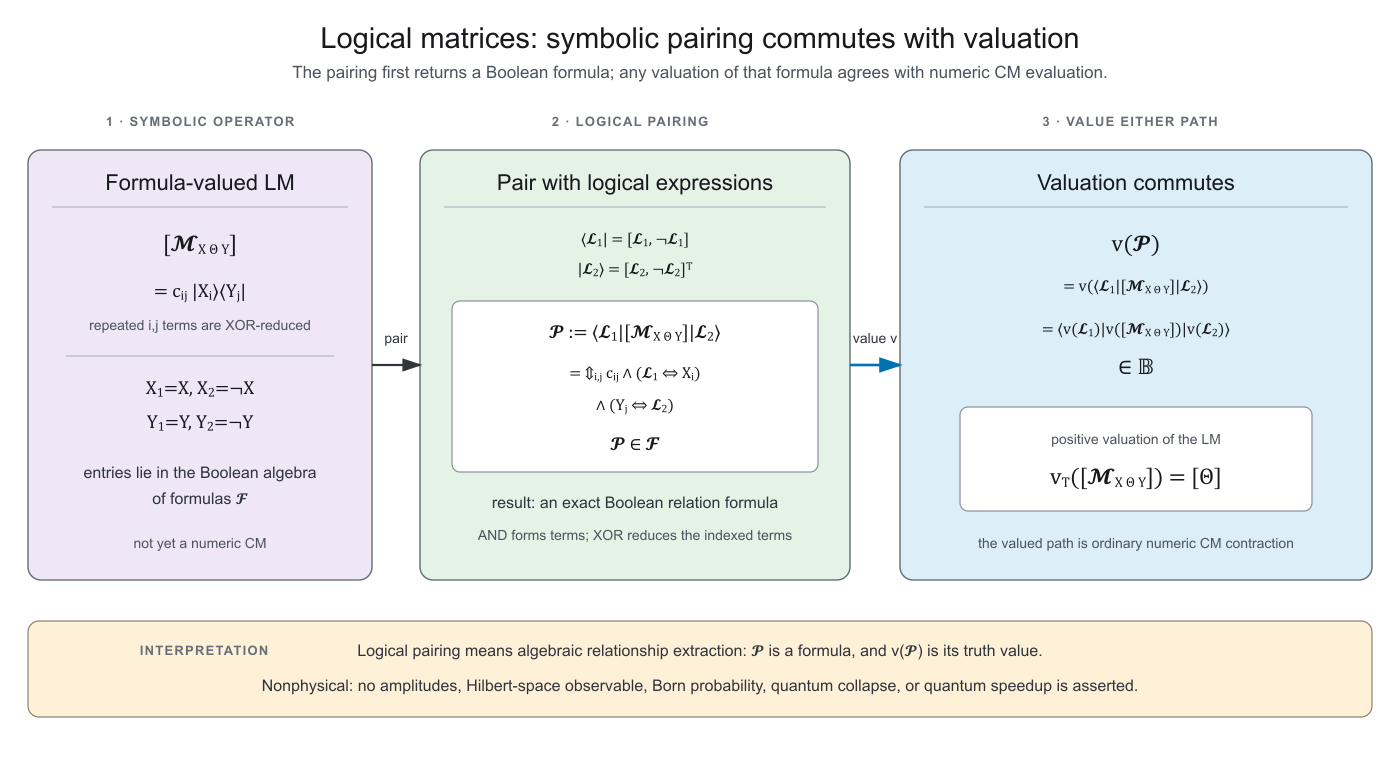
\includegraphics[width=\textwidth]{figure_04_lm_valuation_and_pairing_preview.png}
  \caption{A formula-valued LM is paired with logical expressions before or
  after valuation. Because valuation is a Boolean-algebra homomorphism, both
  paths give the same truth value. Logical pairing denotes algebraic
  relationship extraction, not a physical measurement process.}
  \label{fig:lm-valuation}
\end{figure}

For a formula $A\in\Formula$, define
\begin{equation}
  \stateket{A}=\begin{bmatrix}A\\\neg A\end{bmatrix},
  \qquad
  \statebra{A}=\begin{bmatrix}A&\neg A\end{bmatrix}.
\end{equation}
The XOR--AND contraction of two such states gives logical equivalence:
\begin{equation}
  \statebra{A}\stateket{B}
  =(A\wedge B)\XOR(\neg A\wedge\neg B)
  =(A\Leftrightarrow B).
  \label{eq:logical-inner-product}
\end{equation}
For arbitrary formulas $\mathcal{L}_1$ and $\mathcal{L}_2$, define the logical
pairing
\begin{align}
  \mathcal{P}
  &:=\statebra{\mathcal{L}_1}
      [\mathcal{M}_{X\Theta Y}]
      \stateket{\mathcal{L}_2} \\
  &=\mathop{\XOR}_{i,j\in\{1,2\}}
    c_{ij}\wedge(\mathcal{L}_1\Leftrightarrow X_i)
    \wedge(Y_j\Leftrightarrow\mathcal{L}_2).
  \label{eq:logical-pairing}
\end{align}
The output $\mathcal{P}\in\Formula$ has an exact semantic form.
\begin{proposition}[Logical-pairing identity]
For every $A,B\in\Formula$,
\begin{equation}
  \statebra{A}[\mathcal{M}_{X\Theta Y}]\stateket{B}
  \equiv
  (A\Leftrightarrow X)\mathbin{\Theta}(Y\Leftrightarrow B).
  \label{eq:logical-pairing-identity}
\end{equation}
\end{proposition}
For example, setting $A=X$ and $B=Y$ makes both equivalence factors true, so
the pairing evaluates the declared coefficient $1\mathbin{\Theta}1=\Theta_{11}$.
More generally, the equivalence factors state which polarities of the two
operands are presented to $\Theta$; the full proof is in the appendix.

\begin{theorem}[Valuation commutes with LM pairing]
For every Boolean-algebra valuation $v$,
\begin{equation}
  v(\mathcal{P})
  =\statebra{v(\mathcal{L}_1)}
     v\!\left([\mathcal{M}_{X\Theta Y}]\right)
     \stateket{v(\mathcal{L}_2)}.
  \label{eq:valuation-commutes}
\end{equation}
\end{theorem}

\begin{proof}
The finite pairing in \eqref{eq:logical-pairing} is built only from
negation, conjunction, and exclusive-or. A Boolean valuation preserves each
of these operations, so it can be moved through every term and through the
finite XOR reduction.
\end{proof}

The primary term in this paper is \emph{logical pairing}. The historical word
\emph{measurement} refers only to extracting a coefficient or relationship
from a symbolic operator. No amplitudes,
Hilbert-space observable, Born probability, physical state collapse,
entanglement, or quantum speedup is asserted. Operator and bra--ket notation
also appears in explicitly quantum-adjacent logical formalisms such as
Eigenlogic \citep{toffano2015,duboistoffano2016}; those formalisms include
mathematical structures that are absent here. Figure~\ref{fig:lm-valuation}
makes the nonphysical interpretation explicit.

}

\section{Compiler method}
\label{sec:compiler}

\subsection{Five artifacts, not one}

The implementation contains several objects that can all appear informally as
\enquote{a CM}. Treating them as interchangeable would make both correctness
and timing claims ambiguous. Table~\ref{tab:artifacts} fixes the terminology
used in the remainder of the paper.

\begin{table}[H]
  \centering
  \small
  \begin{tabular}{@{}L{0.20\linewidth}L{0.34\linewidth}L{0.19\linewidth}L{0.17\linewidth}@{}}
    \toprule
    Artifact & Meaning & Size/order & Role \\
    \midrule
    CM operator token &
      One binary truth function packed into four bits &
      $(11,10,01,00)$; true-first &
      Constant-size transform and fusion \\
    Pair surrogate &
      Token plus canonical row and column variable names &
      One ordered variable pair &
      Carries the operand-frame invariant \\
    CM IR &
      Interned Boolean expression DAG &
      False-first array axes &
      General symbolic fallback and compilation \\
    Flat program &
      Instruction sequence compiled from the CM IR &
      Backend-dependent &
      Repeated packed or array evaluation \\
    Explicit CM &
      Dense truth-relation array over declared row/column variables &
      $2^n$ entries; false-first &
      User-visible materialized output \\
    \bottomrule
  \end{tabular}
  \caption{Implementation artifacts and their declared semantic boundaries.
  Only the first is the constant-size binary operator of
  \cref{sec:cm-operators}.}
  \label{tab:artifacts}
\end{table}

The token is the paper's compact binary operator. The pair surrogate gives that
token a frame. The IR and flat program preserve expression structure for more
general formulas, whereas an explicit CM materializes the complete requested
truth relation. Each benchmark endpoint therefore names the artifact it
returns; a token-only endpoint cannot be reported as though it had already
paid for an explicit $2^n$-entry output.

\subsection{Signed-pair implementation}

The implementation enforces the disjoint-layout and distinct-variable
admissibility conditions stated in \cref{sec:alignment-fusion}. For a valid
request it constructs a result satisfying \eqref{eq:pair-invariant} through
the following ordered cases.

\begin{enumerate}
  \item A supported binary connective over two signed literals is recognized.
  Finite negation chains determine each literal's polarity. Operand exchange
  becomes transpose, and negative row or column literals become the
  corresponding permutations from \eqref{eq:frame-transformations}.
  \item Negation of an already compiled pair complements the four token bits.
  \item Two child pairs are combined only when both canonical row/column names
  agree. Their outer connective is then applied through a fixed entrywise
  lookup table, implementing \eqref{eq:same-operands-fusion}.
  \item If structural construction stops but the remaining subtree has exactly
  one live row variable and one live column variable, the compiler evaluates
  its four assignments and places the results in true-first token order. This
  is \emph{local pair retabulation}. If a parent later negates or fuses this
  result, the root is explicitly classified as hybrid rather than purely
  structural.
  \item If none of these cases applies, the expression remains on the ordinary
  CM-IR path.
\end{enumerate}

The public API exposes three strategies. \texttt{pure\_structural} permits
only Cases 1--3; \texttt{hybrid} also permits Case 4; and
\texttt{retabulate} bypasses recursive assembly and evaluates the entire root
on four assignments. Every call records exactly one root outcome:
\texttt{pure\_structural}, \texttt{hybrid\_pair},
\texttt{full\_retabulation}, or \texttt{ordinary\_fallback}. The former
\texttt{structural} API spelling remains only as a reported compatibility alias
for \texttt{hybrid}; it is not used as an experimental arm name.

\paragraph{Compact algorithm.}
For a node $e$, \textsc{Pair}$(e,\Gamma,\mathit{allowRetab})$ first attempts a
signed primitive. It then recursively attempts token negation or same-frame
binary fusion. If those fail and $\mathit{allowRetab}$ is true, it checks that
the live support is exactly $\{R,C\}$ and retabulates that subtree. Otherwise it
returns no pair. The caller converts no-pair to ordinary IR and assigns root
provenance from the returned pair's structural-step and retabulated-subtree
flags. This executable ordering implements the judgments in
\eqref{eq:pair-judgment}--\eqref{eq:pair-rules}.

\paragraph{Worked compiler trace.}
Let
$e=(X\Rightarrow\neg Y)\XOR(\neg Y\Rightarrow X)$ with canonical frame
$(X,Y)$. The left implication becomes token $0111_2$ after a column-polarity
swap. The right implication becomes $1110_2$ after operand exchange and the
corresponding polarity alignment. Both children now carry identical $(X,Y)$
metadata, so entrywise XOR returns $1001_2$, the XNOR token. The trace records
two primitive tokens, two signed alignments, one fusion, zero retabulations,
and root outcome \texttt{pure\_structural}. Had either child required local
retabulation, the same final fusion would instead be labeled
\texttt{hybrid\_pair}.

The supported primitive connectives are AND, OR, XOR, implication, and
equivalence. Primitive operands may have any finite stack of negations and may
arrive in row/column or column/row order. Recursive pair construction supports
negation and the same five connectives when the child metadata match. The
structural claim does not cover two arbitrary compound formulas treated as
opaque operands, equivalence discovery between compound operands, or fusion
across different row/column partitions.

Every recursive pair call receives a strict AST child, so structural
compilation terminates for finite expressions. Retabulation performs four
finite evaluations. For fixed $R$, $C$, and true-first order, the returned
four-bit token is canonical for its binary truth function; neither the source
syntax nor the surrounding IR is claimed to be globally canonical.

\subsection{Layout conversion, ownership, and cost}

The compact token and dense array deliberately use different historical
orders. Before lifting a token, the implementation reverses both token axes:
if $T$ is true-first and $D$ is the false-first $2\times2$ view, then
\begin{equation}
  D_{ab}=T_{1-a,1-b},
  \qquad a,b\in\{0,1\}.
  \label{eq:layout-conversion}
\end{equation}
Axes absent from the pair are then broadcast into the requested variable
layout. The returned dense array is an owned copy; it does not expose a
writable broadcast view. Expression nodes and pair surrogates are immutable,
tokens are integers, and caller-owned layout and fixed-assignment inputs are
read-only under the pair compiler's contract.

Let $N$ be the number of AST occurrences, $U$ the number of unique DAG nodes,
$H$ the AST height, $S$ the number of occurrences in a subtree sent to
retabulation, $D$ that subtree's evaluation depth, $k$ the length of a signed
literal's negation chain, and $n$ the number of requested unfixed Boolean
output axes. Inspecting a signed literal costs $O(k)$, followed by an $O(1)$
four-bit alignment transform; token fusion itself is $O(1)$. One retabulation
uses $O(4S)$ time and $O(D)$ evaluation-stack space. A fully successful
structural pair tree is ordinarily $O(N)$ time and $O(H)$ stack space, although
the current support-discovery implementation can rescan nested rejected
subtrees and has an $O(N^2)$ worst case. A sharing-aware evaluator may instead
scale with $U$, which is why it is a required comparator. Most importantly,
lifting any method to a complete explicit result costs $\Theta(2^n)$ time and
output space.
Constant-time token fusion is therefore a kernel property, not an end-to-end
complexity claim.

The compiler records AST occurrences, unique object nodes, AST height, pair
compiler calls, scanned negation nodes, primitive tokens, signed alignments,
token negations, token fusions, local retabulations, attempts, collapses, and
the root outcome. The legacy \texttt{pairable\_ratio} is retained for old
result readers but is not compared across strategies because their traversals
differ. These diagnostics describe mechanism; they do not substitute for
elapsed time, peak memory, or a sharing-aware comparison.

\subsection{Verification boundary}

The current finite suite covers all 16 tokens in all eight signed operand
frames, all five primitive connectives in those frames, recursive fusion after
alignment, pure-versus-hybrid provenance, direct retabulation, fixed
substitutions in the direct packed comparator, true-first constants, 250 seeded
random two-variable formulas, public token-only behavior, and input
nonmutation. The focused pair, optimization, output-budget, and packed-backend
suites contain 116 passing tests.
Independent exhaustive checks also cover 1,048,576 signed-alignment/fusion
cases. These checks strengthen implementation assurance; they do not replace
the soundness proof, prove unbounded complexity claims, or establish a speed
advantage.

\subsection{Availability and reproducibility}

The review artifact includes the LaTeX source and proof appendix, the pair
compiler and packed comparator, the finite checker, tests, and evaluation
protocol v3. From the repository root, the focused suite uses
\texttt{python -m pytest -q} with these four files:
\begin{quote}\small
  \path{tests/test_cm_pair_alignment.py}\\
  \path{tests/test_cm_optimizations.py}\\
  \path{tests/test_output_budget.py}\\
  \path{tests/test_bitset_backend.py}
\end{quote}
Manuscript notation and citation checks use \texttt{python} with
\path{paper_program/05_manuscript/check_manuscript.py}. The
confirmatory package must additionally contain the content-addressed source
snapshot, environment capture, corpus provenance and licenses, exact command,
schedule, and append-only observations required by protocol v3. A public
repository or archival supplement identifier remains required before
submission and will replace this review-package description.

\relatedworksection
\logicalmatrixsection

\section{Experimental method}
\label{sec:experiments}

The confirmatory evaluation is designed around a conditional question: where,
if anywhere, does operand-aligned token compilation reduce user-visible cost?
All arms consume the same immutable AST and declared variable order. Separate
CM arms request pure structural construction, hybrid construction with local
retabulation, and whole-root retabulation; ordinary fallback is a recorded
outcome rather than a successful pair. They are compared with the ordinary CM
IR, a direct identity-memoized packed evaluator of the source DAG, a lowered
sharing-aware packed program for prepared reuse, an ROBDD with declared
variable order \citep{bryant1986}, and a mandatory ABC-compatible AIG flow for
the frozen translatable-circuit subset. If that AIG environment cannot be
frozen, the circuit campaign is not confirmatory under protocol v3. A four-bit
query calls the same \texttt{cm\_token\_value} implementation after either
producer returns the same word. NPN canonicalization is recorded only when the
synthesis flow invokes it; it is neither charged to CM nor presented as an
evaluation algorithm. Backend-native preprocessing is timed and reported.

For the direct two-variable packed arm, assignment bit positions are
$(00,01,10,11)$ from least to most significant. The row and column masks are
therefore $1100_2$ and $1010_2$, respectively. One memoized traversal applies
the source connectives as machine-bit operations and returns a four-bit truth
word; read most-significant bit first, that word is exactly the CM token order
$(11,10,01,00)$. This baseline does not construct a $2\times2$ array, perform
four separate scalar traversals, or use CM alignment rules. Fixed variables are
represented by all-zero or all-one masks under the same interface. Cold
one-shot measurements clear the environment cache and include mask
construction; prepared measurements build it once and report that preparation
separately. This baseline is consequently
the closest direct test of whether structural pair recognition saves work over
ordinary bit-parallel truth-table evaluation \citep{lee2022}.

\subsection{Workloads and endpoints}

The generated corpus separates exact-frame formulas, signed or swapped frames,
two-variable retabulation cases, hybrid mixed-child cases, formulas involving
multiple operand pairs, compound-operand cases outside the structural claim,
and untouched natural formulas or circuits. Balanced trees use AST occurrence
counts $15,63,255,1023,4095$; skewed trees use $15,63,255$ and must have measured
height at most 128. Larger skewed cells are excluded by design rather than
allowed to fail at the host-language recursion limit. Every in-scope recursion
failure remains an observation. Generated cells also cross all five outer
connectives, reuse counts $1,10,100,1000$, and three sharing conditions:
identity-shared DAG nodes, structurally equal but separately allocated
subtrees, and no sharing. Each case records both AST occurrences $N$ and unique
object nodes $U$. Requested outputs include the compact token, scalar
evaluation, packed batches, and explicit dense CMs where the output budget
permits them. Fixed-substitution cases form a prespecified correctness and
secondary-timing set; the sole primary cell has no fixed variables.

Before any natural case is compiled, the freeze records its source repository
and revision, license, extraction and exclusion rules, original circuit or
formula identifier, size, support distribution, structural duplication,
identity sharing, and translation hash. Semantic duplicates are retained only
as separately identified source structures. The ABC-compatible tool version,
commands, library inputs, and supported circuit subset are part of the same
immutable manifest.

The primary endpoints are one-shot end-to-end time, prepared repeated-
evaluation time, and peak process memory above a pre-run baseline. Each arm
uses a named timing boundary: structural recognition plus token construction;
four complete scalar traversals for retabulation; one packed AST traversal;
lowering plus packed-program execution; token/LUT query after preparation; and
conversion plus allocation for any explicit dense result. Preparation and
query time are never pooled silently. In particular, once either method has
the same four-bit token, its LUT query is identical; any advantage must arise
before that common endpoint or from a measured reuse policy.

Endpoints are reported separately by workload stratum, output type, reuse
count, sharing condition, and root outcome. Mechanism diagnostics include
token-only compilation, support discovery, conversion and allocation, AST
occurrences, unique nodes, AST height, compiler calls, negation scans,
speculative and successful pair constructions, local retabulations, root
provenance, representation size, explicit output bytes, exceptions, timeouts,
and budget rejections. Break-even reuse is computed from measured preparation
and per-evaluation costs rather than extrapolated from the four-bit kernel.

\subsection{Correctness and sampling}

Correctness is checked before performance results are summarized. Completed
arms must agree with an independent truth-table oracle whenever exhaustive
evaluation fits the output budget; larger cases use a frozen random assignment
set and an independent equivalence check where available. Inputs must remain
unchanged. Every disagreement, exception, timeout, or rejection remains in the
raw results with its case identifier and disposition.

Measurements run in isolated processes on a recorded software and hardware
environment. Correctness and one untimed warm-up precede sampling. Arm order is
randomized within each case using a recorded schedule seed. Generated cells
receive at least 30 valid repetitions and natural cases at least 15 unless the
predeclared 60-second timeout intervenes. Timed inner loops last at least
100 milliseconds when repeated evaluation is semantically appropriate. Peak
memory is measured in a fresh process without subtracting undeclared caches.

For paired comparisons, the analysis reports median absolute time, competitor-
to-CM time ratio, median memory difference, case-level distributions, and a
95\% hierarchical bootstrap interval resampling cases and repetitions. A
practical positive region has one primary utility cell: signed/permuted
Stratum B, balanced $N=1023$ formulas with $U=N$, no fixed variables, compact
token output, reuse count one, and root outcome
\texttt{pure\_structural}, compared end to end with the direct packed-AST arm.
Stratum B is generated from the pure structural grammar; an observed non-pure
root is a correctness-gate failure and is not excluded from the primary cell.
Success requires zero correctness disagreements, a median competitor-to-CM
time ratio of at least $1.20$ with its 95\% interval entirely above one, and no
more than a 10\% median peak-memory increase. The 20\% effect is the minimum
considered practically worthwhile and is four times the protocol's target 5\%
relative repeatability bound; the 10\% memory tolerance accommodates allocator
granularity without accepting a material space tradeoff. A pilot that cannot
meet the repeatability bound forces a successor protocol rather than a changed
threshold. Structural-versus-retabulation and every other cell are secondary,
with multiplicity controlled within endpoint families. Falling below the sole
primary rule narrows the result; it does not justify selecting another cell
after the fact.

Protocol v3, source state, corpus, seeds, arm configuration, schedule,
environment, test output, and append-only raw observations are content-hashed
before the first confirmatory run. Any substantive change produces a new
protocol version. This freeze keeps the empirical claim separate from the
examples used to develop the compiler.

\section{Results and evidence status}
\label{sec:results}

The formal and implementation evidence currently clears the following
pre-performance gates: exhaustive token and signed-frame checks, exhaustive
signed alignment/fusion enumeration, randomized two-variable differential
checks, and public-API tests for pure structural, hybrid, whole-retabulation,
fallback, output, fixed-substitution, and input-ownership behavior. These
results support correctness of the tested
implementation surface; they do not establish a runtime or memory advantage.

No confirmatory performance table or Figure~5 appears in this working draft.
The corpus and run manifest have not yet been frozen and the campaign has not
been executed. Quantitative speed, memory, break-even, prevalence, and failure-
region claims therefore remain open. Kernel-only timings and previously
superseded headline speedups will not be reused as end-to-end results. This is
an explicit evidence boundary rather than a missing positive result: the final
section will report every frozen arm and stratum, including ties, losses,
timeouts, and cases in which pair recognition falls back.

\section{Discussion and limitations}
\label{sec:discussion}

The explicit representation of an arbitrary $n$-variable Boolean function
contains $2^n$ truth values. It may be written as an order-$n$ tensor of side
two, a length-$2^n$ vector, or, after an even split of $2m$ variables, a
$2^m\times2^m$ matrix. No reshape removes this worst-case output size.
Compression and symbolic sharing must therefore be evaluated separately.

Operator fusion also depends on repeated, alignable operands. When compatible
pairs are rare, when normalization dominates, or when another representation
preserves substantially more sharing, the CM path may tie or lose. These are
expected boundary cases, not failures to be hidden. The final discussion will
interpret them together with preparation cost, memory traffic, reuse count,
variable ordering, and fallback frequency.

\section{Conclusion}
\label{sec:conclusion}

Correspondence matrices are best understood as typed Boolean operators rather
than as a novelty claim about reshaped truth tables. XOR--AND contraction lets
one-hot operand states evaluate those operators; matrix transformations align
signed operand frames; and exact compatible frames can be fused before
evaluation. Formula-valued logical matrices add a symbolic layer whose
valuation recovers numeric CMs and whose logical pairing remains within
Boolean algebra. The remaining empirical question is deliberately practical:
which workloads permit this operator-level rewrite to reduce total computation
after all costs are counted?

\appendix

\section{Proof details}
\label{app:proofs}

This appendix collects the typed arguments supporting the concise statements
in the main text. All scalar sums are XOR reductions and all scalar products
are conjunctions unless another algebra is named explicitly.

\subsection{Representation and selection}

\begin{proposition}[Unique binary representation]
The map from a binary Boolean operator $\Theta$ to $\CM{\Theta}$ is a
bijection between functions $\Bool^2\rightarrow\Bool$ and matrices in
$\Bool^{2\times2}$ once the row, column, and truth-state order is fixed.
\end{proposition}

\begin{proof}
A binary Boolean function is determined by its four values on
$(1,1),(1,0),(0,1),(0,0)$. These are exactly the four entries of
$\CM{\Theta}$. Conversely, any four-bit matrix assigns one output to each
binary input pair and therefore defines one such function. Both sets contain
$2^4=16$ elements.
\end{proof}

For completeness, expand the contraction as
\begin{equation}
  E_{\CM{\Theta}}(x,y)
  =\mathop{\XOR}_{r,s\in\{1,0\}}
    \chi_x(r)\wedge\Theta_{rs}\wedge\chi_y(s),
  \qquad
  \chi_z(q):=\begin{cases}1,&q=z,\\0,&q\ne z.\end{cases}
\end{equation}
The two one-hot states make
$\chi_x(r)\wedge\chi_y(s)$ equal to one only at $(r,s)=(x,y)$.
This proves selection without a cancellation or distributivity assumption
beyond the declared Boolean algebra. It also explains why OR--AND selection
would return the same scalar on one-hot states, although OR does not supply the
same coefficient-space algebra for arbitrary vectors.

\subsection{Coefficient linearity and basis}

For fixed $x,y$, distribute conjunction over XOR:
\begin{align}
  E_{A\XOR B}(x,y)
  &=\mathop{\XOR}_{r,s}
    \chi_x(r)\wedge(A_{rs}\XOR B_{rs})\wedge\chi_y(s) \\
  &=E_A(x,y)\XOR E_B(x,y).
\end{align}
Thus evaluation is a coordinate projection and hence a linear functional on
$\GFtwo^{2\times2}$. Let $E_{rs}$ be the matrix with a one only at position
$(r,s)$. Evaluating
\begin{equation}
  \CM{\Theta}=\mathop{\XOR}_{r,s}\Theta_{rs}E_{rs}
\end{equation}
at any position selects $\Theta_{rs}$, proving the basis decomposition and
coefficient extraction. This proof concerns the coefficient matrix. The
affine truth-state encoding prevents it from implying that every represented
Boolean function is linear in its logical inputs.

\subsection{Signed operand transformations}

Let $P=\begin{bmatrix}0&1 \\ 1&0\end{bmatrix}$. The row-$x$, column-$y$
entry of $P\CM{\Theta}$ is the row-$\neg x$, column-$y$ entry of
$\CM{\Theta}$ and is therefore $(\neg x)\mathbin{\Theta}y$. Similarly,
right multiplication by $P$ exchanges the column assignment and
transposition exchanges the two input assignments. With
$\Theta^\tau(x,y):=\Theta(y,x)$, hence
\begin{align}
  \CM{\Theta^\tau} &= \CM{\Theta}^{\mathsf T}, &
  \CM{\Theta(\neg X,Y)} &= P\CM{\Theta}, \\
  \CM{\Theta(X,\neg Y)} &= \CM{\Theta}P, &
  \CM{\Theta(\neg X,\neg Y)} &= P\CM{\Theta}P.
\end{align}
Negating every output flips every bit, which is entrywise XOR with the
all-ones matrix. Products with $P$ are XOR--AND products, but only one entry
survives in each output position, so they can equivalently be implemented as
direct permutations.

For XNOR, $\CM{\Leftrightarrow}$ is the identity matrix. Under the explicit
clockwise convention
$\operatorname{rot}_{90^\circ}\!\begin{bmatrix}a&b\\c&d\end{bmatrix}
=\begin{bmatrix}c&a\\d&b\end{bmatrix}$, its ones move to the antidiagonal,
giving $\CM{\XOR}$. (For this particular symmetric matrix, counterclockwise
rotation gives the same result.) The two supports are disjoint and cover all four
positions, so their entrywise XOR is the all-ones $\CM{\impax}$.

\subsection{Operand-aligned fusion}

Let $\Phi$ be any binary Boolean operator and define
\begin{equation}
  F_{rs}:=(\Theta_1)_{rs}\mathbin{\Phi}(\Theta_2)_{rs}.
\end{equation}
When both inner operators use the same operand frame, selection gives
\begin{align}
 &(x\mathbin{\Theta_1}y)\mathbin{\Phi}
   (x\mathbin{\Theta_2}y) \\
 &\qquad=(\Theta_1)_{xy}\mathbin{\Phi}(\Theta_2)_{xy}
 =F_{xy}
 =\statebra{x}F\stateket{y}.
\end{align}
No general distributive law for $\Phi$ over XOR is used. If the original
operators differ by signed operand order, the preceding transformations first
translate each one into the target frame; applying the same argument after
that translation proves fusion after alignment.

For pure structural compilation, proceed by induction on the derivation of
$\Gamma\vdash e\Downarrow^{\mathsf S}\operatorname{Pair}(R,C,t)$. A primitive
signed-literal pair is sound by the transformations above. For the unary step,
complementing all four token bits implements logical negation. For the binary
step, the induction hypotheses give two sound child pairs in the same typed
frame, and the preceding entry-selection calculation proves their entrywise
outer-connective fusion. Every recursive call visits a strict AST child,
proving termination. This establishes structural soundness without using
retabulation.

For exact pair retabulation, evaluate the subtree independently at
$(1,1),(1,0),(0,1),(0,0)$ and store the four observed bits in that order.
Selection at any assignment returns the stored value by construction. The
whole-root retabulation is therefore sound. For a hybrid derivation, induct on
the judgment in \eqref{eq:pair-judgment}. The new base case is an exactly
retabulated subtree. Every negation or fusion above that base preserves the
invariant by the same unary and binary arguments used for pure structural
compilation. Provenance changes the reported construction class, not the
invariant. The top-level compiler consequently returns only a pure structural
pair, a whole-root retabulation, a hybrid pair assembled from sound children,
or the ordinary IR result. The ordinary IR retains responsibility for every
expression not admitted by a pair judgment.

\subsection{Formula-valued LMs}

Let $B_{ij}(X,Y)=\otbktwo{X_i}{Y_j}$. The upper-left cell of
\begin{equation}
  [\mathcal{M}_{X\Theta Y}]
  =\mathop{\XOR}_{i,j\in\{1,2\}}c_{ij}B_{ij}(X,Y),
  \qquad c_{ij}:=\Theta_{b_i b_j},\quad b_1=1,\ b_2=0,
\end{equation}
is the disjoint-minterm expansion
\begin{equation}
  c_{11}XY
  \XOR c_{12}X\neg Y
  \XOR c_{21}\neg X Y
  \XOR c_{22}\neg X\neg Y.
\end{equation}
Under the declared position-to-assignment map, this is
$X\mathbin{\Theta}Y$. Exchanging the $Y$ components gives
$X\mathbin{\Theta}\neg Y$; exchanging the $X$ components gives
$\neg X\mathbin{\Theta}Y$; and exchanging both gives the lower-right
formula. This proves the polarity-orbit form in \eqref{eq:lm-matrix}.

If $v(X)=x$ and $v(Y)=y$, applying $v$ to those four formulas either preserves
or exchanges the two row and column assignments. It follows that
\begin{equation}
  v([\mathcal{M}_{X\Theta Y}])
  =P^{1-x}\CM{\Theta}P^{1-y}.
\end{equation}
The positive case $x=y=1$ yields $\CM{\Theta}$.

For formulas $A,B$,
\begin{equation}
  \statebra{A}\stateket{B}
  =(A\wedge B)\XOR(\neg A\wedge\neg B)
  =(A\Leftrightarrow B),
\end{equation}
because the two conjunctions are disjoint. Substituting the LM basis expansion
between $\statebra{\mathcal L_1}$ and $\stateket{\mathcal L_2}$ and using this
identity on both sides of each outer product gives
\begin{equation}
  \mathop{\XOR}_{i,j}
    c_{ij}\wedge(\mathcal L_1\Leftrightarrow X_i)
    \wedge(Y_j\Leftrightarrow\mathcal L_2).
\end{equation}
For each valuation of $A,B,X,Y$, exactly one $i$ satisfies
$A\Leftrightarrow X_i$ and exactly one $j$ satisfies
$Y_j\Leftrightarrow B$. If these positions are $i^*,j^*$, the XOR therefore
selects $c_{i^*j^*}=\Theta_{b_{i^*}b_{j^*}}$. By the definitions of the
polarity orbit and $b_i$ under this valuation,
$b_{i^*}=v(A\Leftrightarrow X)$ and
$b_{j^*}=v(Y\Leftrightarrow B)$. Hence the selected coefficient equals
$v((A\Leftrightarrow X)\mathbin{\Theta}(Y\Leftrightarrow B))$. This holds for
every valuation, proving \eqref{eq:logical-pairing-identity}.

Finally, a Boolean valuation is a homomorphism for negation, conjunction, and
XOR. Moving it through this finite expression term by term proves
\eqref{eq:valuation-commutes}.

\subsection{ANF conversion is a different map}

For $n$ variables, identify a valuation with its support
$S\subseteq\{1,\ldots,n\}$ and let $t_S$ be the corresponding truth value.
If
\begin{equation}
  f(x_1,\ldots,x_n)
  =\mathop{\XOR}_{T\subseteq\{1,\ldots,n\}}
    \left(a_T\wedge\bigwedge_{i\in T}x_i\right),
\end{equation}
then evaluation on support $S$ gives
\begin{equation}
  t_S=\mathop{\XOR}_{T\subseteq S}a_T.
\end{equation}
Boolean M\"obius inversion gives the converse relation
\begin{equation}
  a_T=\mathop{\XOR}_{S\subseteq T}t_S.
\end{equation}
Thus ANF coefficients arise by an invertible coordinate transform of the truth
vector. By contrast, positive valuation maps the formula-valued polarity orbit
directly to a numeric CM. The two maps have different domains and purposes
even though both ultimately describe the same Boolean function.

\subsection{Higher-arity size}

An arbitrary function of $n$ Boolean variables has one output for each of
$2^n$ valuations. Its explicit operator therefore has $2^n$ bits. The same
data can be placed in an order-$n$ tensor with side length two, a
length-$2^n$ vector, or, after splitting $2m$ variables into equal row and
column groups, a $2^m\times2^m$ matrix. These are layout choices with the same
entry count, not compression results.

\section{Finite verification scope}
\label{app:finite-checks}

The accompanying checker exhaustively verifies the 16 binary tokens, 16,384
same-frame fusion cases, 512 signed alignments, 1,048,576 signed
alignment/fusion cases, the XOR/XNOR/Impax identities, LM positive and general
valuations, 256 LM coefficient extractions, 16,384 LM valuation/fusion cases,
and 64 two-variable ANF round trips. Finite enumeration catches convention and
implementation errors but is not used as a proof of an unbounded theorem or a
runtime bound.


\bibliographystyle{plainnat}
\bibliography{references}

\end{document}
